\section{Accelera Pipe Module}

\subsection{Functional Description}

The Accelera Pipe module can be described formally as a directed acyclic graph:
\[
G = (V, E)
\]
where \(V\) is the set of computational nodes and \(E\) is the set of directed dependency
edges between them. Each node \(v_i \in V\) represents one pipeline operation, such as
preprocessing, model fitting, prediction, merging, or metric evaluation. Each edge
\((v_i, v_j) \in E\) means that node \(v_j\) depends on the output of node \(v_i\).
To guarantee valid execution, the graph must satisfy the acyclic condition:
\[
\nexists \; (v_1, v_2, \ldots, v_k) \quad \text{such that} \quad v_1 = v_k
\]

This condition ensures that the graph contains no circular dependencies. Therefore,
the backend can execute the pipeline using a valid topological ordering. If \(\tau(G)\)
denotes a topological order of the graph, then every dependency must appear before
the node that consumes it:
\[
u \rightarrow v \Rightarrow \tau(u) < \tau(v)
\]

During execution, each node applies its stored operation to the outputs received from
its parent nodes. For a node \(v_i\), the output can be represented as:
\[
o_i = f_i(o_{p_1}, o_{p_2}, \ldots, o_{p_m})
\]
where \(f_i\) is the operation stored in the node, and
\(o_{p_1}, o_{p_2}, \ldots, o_{p_m}\) are the outputs of its parent nodes. This
formulation allows both sequential and branched workflows to be handled by the same
execution model.

For branch-based execution, the pipeline may produce several candidate paths. If
\(P = \{p_1, p_2, \ldots, p_n\}\) is the set of candidate paths and \(M(p_i)\) is the
metric value of path \(p_i\), the selected path can be written as:
\[
p^* = \arg\max_{p_i \in P} M(p_i)
\]
for maximization metrics such as accuracy, or:
\[
p^* = \arg\min_{p_i \in P} M(p_i)
\]
for minimization metrics such as loss or error. The selected path \(p^*\) is stored
inside the \texttt{ExecutedGraph}, which keeps only the fitted transformations and
models needed for later inference.

At inference time, the executed graph applies only the selected fitted path to new
input data. If \(X_{\text{new}}\) is the new input, the inference output can be
represented as:
\[
\hat{y} = G^*(X_{\text{new}})
\]
where \(G^*\) is the fitted executed graph selected during training. This separation
reduces unnecessary training-time objects and keeps inference focused on the final
reusable path.

\subsection{Modular Decomposition}

\begin{figure}[H]
\centering
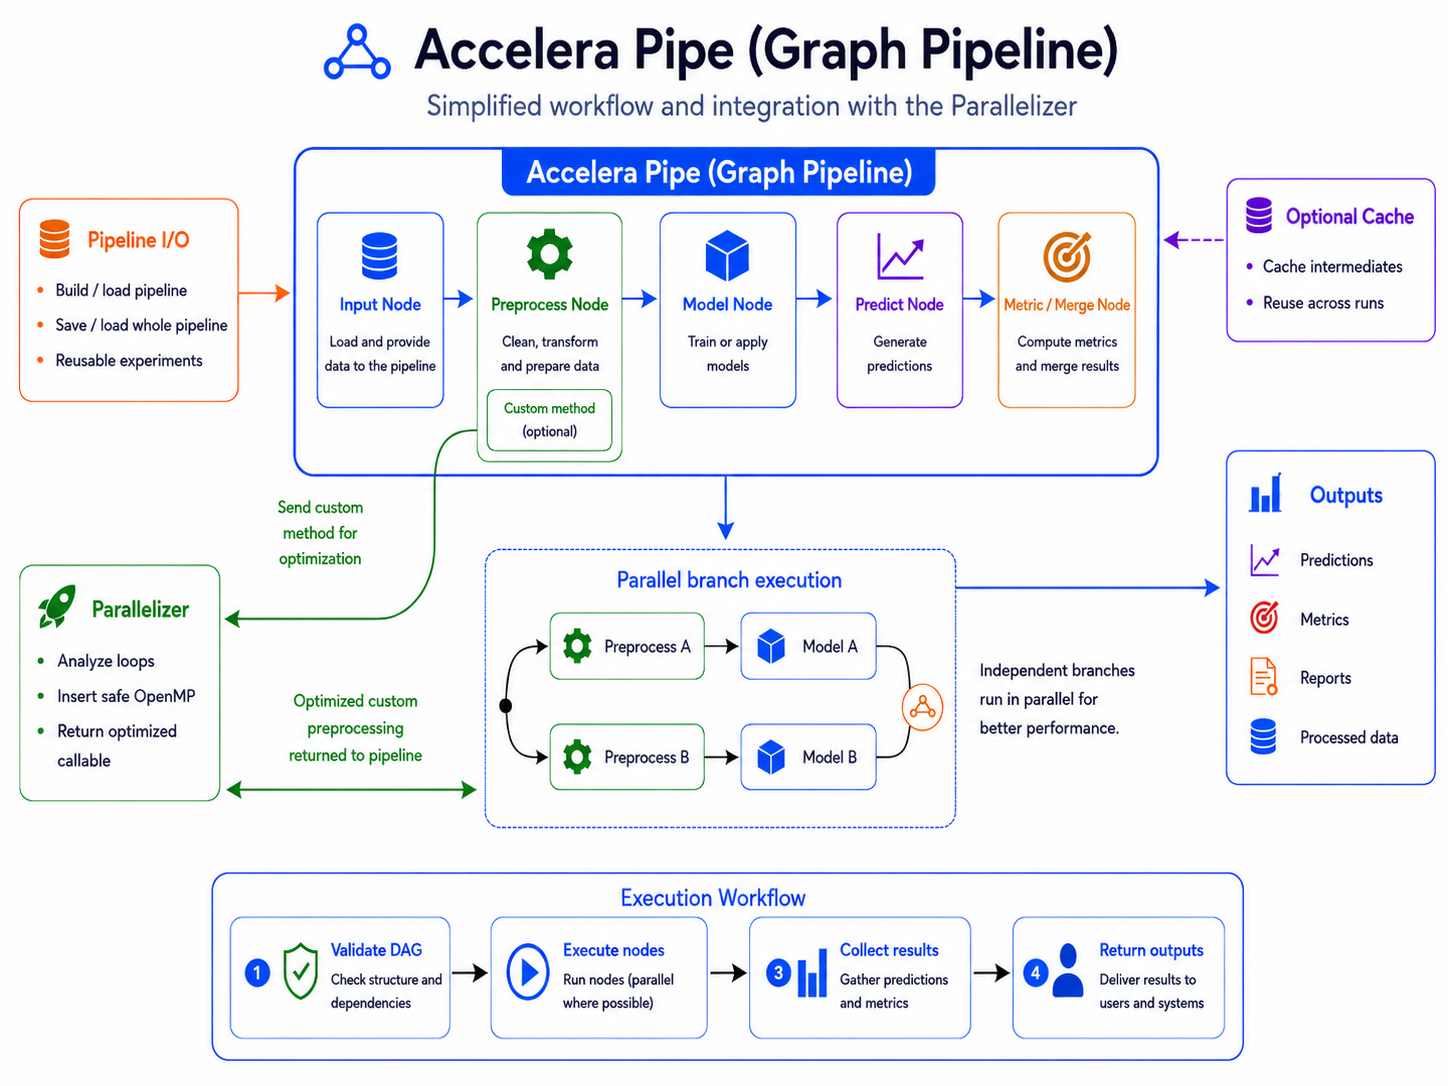
\includegraphics[width=\textwidth,keepaspectratio]{imgs/accelera_pipe.png}
\caption{Accelera Pipe workflow with custom preprocessing parallelization and pipeline reuse.}
\label{fig:accelera-pipe-workflow}
\end{figure}

The Accelera Pipe module is decomposed into two main layers: a Python API layer
and a native C++ graph execution layer. As shown in
Figure~\ref{fig:accelera-pipe-workflow}, the Python layer provides the user-facing
builder interface used to define preprocessing, model, prediction, metric, branch,
and merge nodes. It also handles metric wrapping, reports, serialization, save/load
support, and integration with the Code Parallelizer.

The native C++ layer manages the internal graph representation and execution
behavior. It stores nodes and edges, validates graph connections, computes the
topological execution order, schedules independent branches for parallel execution,
selects the final fitted path, and manages intermediate memory. When a preprocessing
node contains a supported custom method, Accelera Pipe can send it to the
Parallelizer, receive an optimized callable, and attach it back to the graph before
execution.

\begin{table}[H]
\centering
\small
\renewcommand{\arraystretch}{1.15}
\setlength{\tabcolsep}{4pt}
\caption{Main components of the Accelera Pipe module}
\label{tab:accelera-pipe-components}
\begin{tabular}{p{0.30\textwidth}p{0.62\textwidth}}
\toprule
\textbf{Component} & \textbf{Responsibility} \\
\midrule
Pipeline Builder Interface &
Provides the user-facing fluent API used to define preprocessing stages, models,
prediction steps, metrics, merge operations, and branches. It translates each user
call into a typed computational node instead of immediately executing the operation. \\
\midrule
Pipeline State and Persistence Manager &
Owns the native graph object, maps high-level node categories to graph node types,
controls graph execution settings, and provides save/load behavior for reusable
pipeline objects. \\
\midrule
Executed Graph Runtime &
Represents the fitted execution path selected after training. It allows the same
trained transformations and models to be reused for inference without keeping
unnecessary validation data or temporary training branches. \\
\midrule
Metric and Display Wrappers &
Adapt supervised metrics, unsupervised metrics, arrays, figures, dictionaries, and
reports into graph-compatible outputs that can be stored, selected, displayed, or
used in branch-selection strategies. \\
\midrule
Native Graph Engine &
Stores the pipeline as a directed acyclic graph, validates node connections, computes
execution order, schedules sequential or parallel execution, manages branch
selection, and controls intermediate-memory lifetime. \\
\midrule
Node Abstraction Layer &
Defines the common behavior of input, preprocessing, model, prediction, merge, and
metric nodes, including source-node relationships, stored data, GPU usage flags, and
selected-path markers. \\
\bottomrule
\end{tabular}
\end{table}

At the Python API level, each builder method creates or configures one graph
operation. A preprocessing node stores a function or transformer together with
execution parameters such as \texttt{execute\_fit} and \texttt{cache}. Before a
preprocessing function is stored, the module attempts to parallelize it through
\texttt{parallelizer.parallelize}. Model nodes store estimators, prediction nodes
store test data and the prediction method name, metric nodes store metric wrappers,
and merge nodes store the merge strategy.

\begin{table}[H]
\centering
\small
\renewcommand{\arraystretch}{1.15}
\setlength{\tabcolsep}{4pt}
\caption{Mapping from builder calls to graph node semantics}
\label{tab:accelera-pipe-builder-map}
\begin{tabularx}{\textwidth}{p{0.31\textwidth}p{0.18\textwidth}X}
\toprule
\textbf{Builder method} & \textbf{Node type} & \textbf{Main role} \\
\midrule
\texttt{preprocess(name, func)} &
\texttt{PREPROCESS} &
Transform input data or selected columns. \\
\midrule
\texttt{model(name, model)} &
\texttt{MODEL} &
Fit or apply a machine-learning estimator. \\
\midrule
\texttt{predict(name, test\_data)} &
\texttt{PREDICT} &
Run a model output function such as \texttt{predict}. \\
\midrule
\texttt{metric(name, metric)} &
\texttt{METRIC} &
Evaluate predictions using a supervised or unsupervised metric. \\
\midrule
\texttt{merge(name, strategy)} &
\texttt{MERGE} &
Combine outputs from multiple prediction branches. \\
\midrule
\texttt{branch(name, ...)} &
Multiple nodes &
Create alternative candidate paths in the DAG. \\
\bottomrule
\end{tabularx}
\end{table}

\subsection{Branching and Path Selection}

The native backend uses a graph abstraction rather than a linear pipeline. The
\texttt{Graph} class stores all nodes, tracks whether the graph has already been
compiled, supports cloning, and exposes methods for adding nodes, splitting
branches, executing, clearing, saving, loading, and enabling parallel execution.
The graph computes a topological execution order before running. This guarantees
that each node is executed only after its source nodes have produced their outputs.
If the graph contains branches, the execution result is followed by path selection
using one of the supported strategies: maximum metric, minimum metric, custom
strategy, or all paths.

\begin{lstlisting}[style=algostyle,caption={High-level Accelera Pipe training flow},label={alg:pipeline-training-flow}]
Input: training data X, optional labels y, graph G, selection strategy S
Output: predictions or metric results R, executed graph E

1:  Add X and y to the input node of G
2:  Compile G if its topological order is not already available
3:  Execute graph nodes sequentially or in parallel depending on G settings
4:  Collect outputs from final leaf nodes
5:  If G contains branches, select the path requested by S
6:  Clone the selected fitted path into a compact executed graph E
7:  Remove validation-only data and temporary training data
8:  Return R and E
\end{lstlisting}

Branching is handled by the native \texttt{split} operation. Each branch is converted
into a chain of graph nodes starting from the current leaf. If the current leaf node is
\(L\), then a branch \(B_i\) can be represented as:
\[
B_i = (L, n_{i1}, n_{i2}, \ldots, n_{ik})
\]
where \(n_{i1}, n_{i2}, \ldots, n_{ik}\) are the operations added to that branch.
A branch may contain a single node or a list of nodes, so the same mechanism supports
simple model comparison as well as full alternative sub-pipelines.

A useful optimization in branch construction is duplicate first-node sharing. If
several branches begin with the same first node, the graph creates that first node
once and connects the later branch consumers to its output. The sharing condition is:
\[
n_{11} = n_{21} = \cdots = n_{m1}
\]
where \(n_{i1}\) is the first node of branch \(B_i\). This is safe for the first
node because all such branches receive the same original input. The optimization is
deliberately conservative: later repeated nodes are not merged automatically because
their inputs may already differ due to earlier branch operations.

\begin{figure}[H]
\centering
\begin{minipage}{0.49\textwidth}
    \centering
    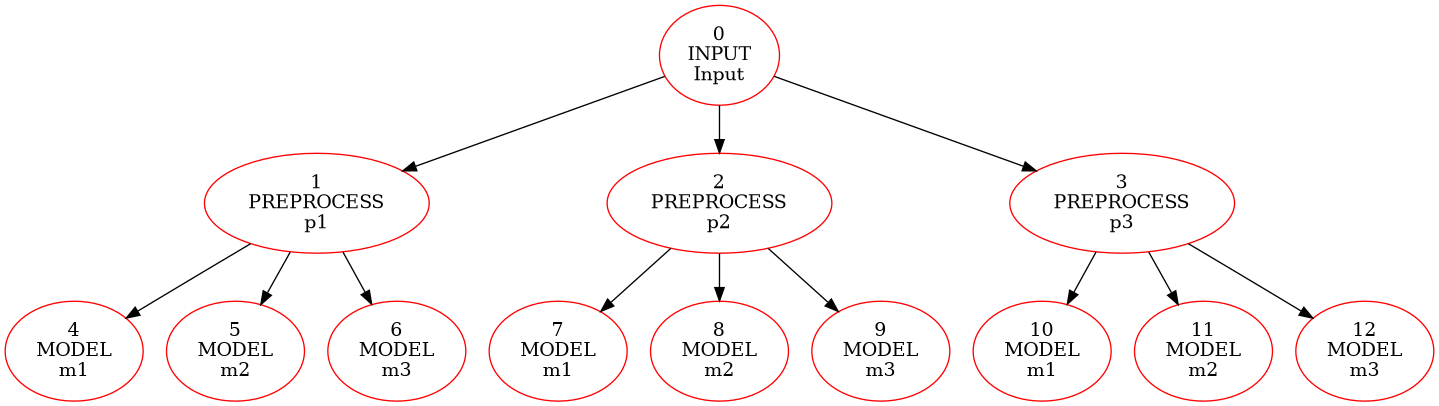
\includegraphics[width=\textwidth]{imgs/before_sharing.png}
    \caption{Before duplicate first-node sharing}
\end{minipage}
\hfill
\begin{minipage}{0.49\textwidth}
    \centering
    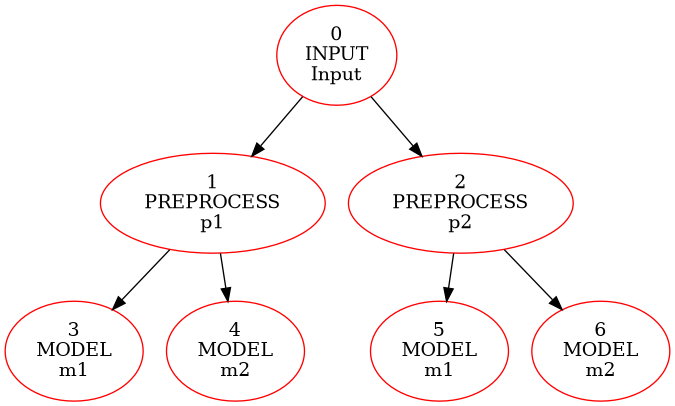
\includegraphics[width=\textwidth]{imgs/after_sharing.png}
    \caption{After duplicate first-node sharing}
\end{minipage}
\end{figure}

\subsection{Intermediate Memory Management}

Machine-learning pipelines can produce large intermediate arrays, especially when
several preprocessing branches are evaluated. Accelera Pipe therefore tracks
remaining consumers for each node output. Once the last downstream consumer finishes,
the corresponding intermediate data can be released. Model and metric nodes are
treated more carefully because they may hold fitted estimators or evaluation state,
while input and preprocessing data can often be cleared after their consumers are
done. This policy reduces memory pressure without changing the logical result of the
graph.

\begin{lstlisting}[style=algostyle,caption={Consumer-count based intermediate release},label={alg:consumer-release}]
Input: executed node N, remaining consumer table C
Output: graph with unused temporary data released

1:  for each source node S that feeds N do
2:      C[S] = C[S] - 1
3:      if C[S] == 0 and S is releasable then
4:          clear the temporary data stored by S
5:      end if
6:  end for
\end{lstlisting}

The consumer-count mechanism is used after each node finishes executing. Every
source node keeps a counter representing how many downstream nodes still need
its output. For a source node \(S\), the remaining-consumer count can be written as:
\[
C(S) = |\{N \mid S \rightarrow N \text{ and } N \text{ has not executed yet}\}|
\]
When a downstream consumer completes, the counter is decreased:
\[
C(S) \leftarrow C(S) - 1
\]
If the counter reaches zero and the source node is safe to clear, the temporary output
is released. This allows the graph to reduce memory pressure during branch-heavy
training runs without changing the final predictions or selected path.

\subsection{Parallel Graph Execution}
The graph can run independent nodes in parallel, but a node can start only after all
its parents have finished. For any node \(N\), the readiness condition is:
\[
\text{ready}(N) \Longleftrightarrow \forall P \in \text{Parents}(N),\; \text{finished}(P)=\text{true}
\]
The backend uses CPU thread semaphores, a separate GPU semaphore, and dependency
checks over the topological order. This prevents a downstream node from reading
incomplete data and also serializes GPU work when necessary. CPU nodes are allowed
to execute concurrently as long as worker slots are available, while GPU nodes are
handled more conservatively using a single execution slot. This makes the scheduler
safe for mixed CPU/GPU graphs without changing the dependency semantics. This also
allows the graph to use available hardware more efficiently when several branches are
ready at the same time. At the same time, synchronization keeps the final execution
result equivalent to a valid sequential topological run. The number of CPU threads is
based on hardware concurrency but can be overridden using the
\texttt{ACCELERA\_NUM\_THREADS} environment variable.

\newpage
\begin{lstlisting}[style=algostyle,caption={Parallel graph execution scheduling},label={alg:parallel-graph-execution}]
Input: topological execution order T
Output: completed graph execution or reported error

1:  Initialize finished and started state for all nodes
2:  Build remaining-consumer counts for intermediate outputs
3:  Create limited CPU worker slots and one GPU execution slot
4:  while unfinished nodes still exist do
5:      for each node N in T do
6:          if N has not started and all parent nodes are finished then
7:              Acquire a CPU slot or the GPU slot depending on N
8:              Mark N as started
9:              Launch N asynchronously
10:             After N finishes:
11:                 Mark N as finished
12:                 Release unused source outputs
13:                 Release the CPU or GPU slot
14:          end if
15:      end for
16:  end while
17:  Wait for all launched tasks
18:  Rethrow any stored node execution error
\end{lstlisting}

Algorithm~\ref{alg:parallel-graph-execution} describes the runtime scheduling idea
implemented by the native graph backend. The graph is already arranged in
topological order, but the scheduler does not simply execute nodes one by one.
Instead, it repeatedly searches for nodes whose parents have finished and launches
them asynchronously when a CPU or GPU execution slot is available. CPU nodes share
a limited pool of worker slots, while GPU nodes use a separate single-slot semaphore
to avoid unsafe concurrent GPU execution. After a node completes, the backend marks
it as finished, releases any temporary source outputs that are no longer needed, and
signals the scheduler so that newly ready child nodes can start. Any exception raised
inside a node is stored and rethrown after all launched tasks are joined, which gives a
clear error message containing the failed node name and whether it was executed as a
CPU or GPU node.


\subsection{Design Constraints}

The Accelera Pipe module has several design constraints that guide how the graph
is constructed, executed, and reused. The first constraint is that the internal
workflow must always remain a valid directed acyclic graph. Since execution
depends on topological ordering, cyclic dependencies are not allowed. For any
edge from node \(u\) to node \(v\), the execution order must satisfy:
\[
u \rightarrow v \Rightarrow \tau(u) < \tau(v)
\]
where \(\tau\) represents the topological order of the graph. This guarantees
that every node is executed only after its required source nodes have already
produced their outputs.

The second constraint is node-type validity. Not every node can be connected to
any other node. For example, a prediction node must follow a model node, a metric
node must follow a prediction or merge node, and a merge node should combine
compatible prediction outputs. These restrictions preserve the semantic meaning
of the pipeline and prevent invalid workflows from reaching the execution stage.

The third constraint is safe memory management. Since branch-heavy workflows can
produce many temporary arrays, the backend must release intermediate data only
when it is no longer needed. For a source node \(S\), the remaining-consumer
count is:
\[
C(S) = |\{N \mid S \rightarrow N \text{ and } N \text{ has not executed yet}\}|
\]
The output of \(S\) can be cleared only when \(C(S)=0\) and the node is safe to
release. This reduces memory pressure without changing the final selected path
or prediction results.

The fourth constraint is parallel execution safety. Independent nodes may run in
parallel, but a node can start only after all of its parent nodes have completed:
\[
\text{ready}(N) \Longleftrightarrow \forall P \in \text{Parents}(N),\;
\text{finished}(P)=\text{true}
\]
This prevents downstream nodes from reading incomplete data. The backend also
uses limited CPU worker slots and a separate GPU slot to avoid unsafe resource
sharing during execution.

Finally, the executed graph must not retain training-only data. After training,
the selected path is cloned into an \texttt{ExecutedGraph}, validation inputs are
removed, metric targets are cleared, and temporary arrays are released. This
keeps the saved inference graph compact and focused only on fitted
transformations and models.


\subsection{Summary}
The Accelera Pipe module also supports persistence. The Python \texttt{PipelineBase}
class saves and loads pipeline objects using pickle, while the C++ graph exposes
its state as a Python dictionary containing node information, selected-path flags,
source indices, cached data, graph compilation state, and parallel execution
configuration. During loading, the graph rebuilds the nodes and reconnects them
using the stored source indices, making the native graph serializable.

The module can also export a graph-like representation of the pipeline structure.
The graph utility code writes an XML-style network description containing layers
for input, preprocessing, model, prediction, merge, and metric nodes, together
with their edges. This representation is useful for debugging, visualization,
and understanding the executable graph generated from the high-level pipeline.

In summary, Accelera Pipe is a hybrid Python/C++ pipeline execution system.
Python provides the user-facing construction interface, while C++ provides graph
semantics, execution scheduling, branch selection, memory-lifetime control, and
parallel execution support, keeping the module both efficient and easy to use.


\section{Code Parallelizer Module}

\subsection{Functional Description}

The Code Parallelizer module is responsible for transforming supported loop-heavy
source code into optimized C++ code annotated with OpenMP pragmas. It is designed
to reduce the execution time of custom preprocessing functions and standalone code
snippets by identifying loops that can be safely executed in parallel. The module
accepts different input forms: a file path, a source string, a custom Python function,
or a custom transformer instance. Regardless of the input form, the scientific goal is
the same: normalize the input into a C++ loop-analysis path, detect parallelization
opportunities, and return either parallelized source code or a compiled
Python-callable native function.

This process can be viewed as a transformation from an original program \(P\) into
an optimized program \(P'\):
\[
P' = \mathcal{T}(P)
\]
where \(\mathcal{T}\) represents the parallelization pipeline, including source
normalization, loop extraction, loop classification, safety validation, and OpenMP
pragma insertion. If no safe optimization is found, the transformation keeps the
program behavior unchanged by returning the original code or callable.

For Python input, the module first lowers a restricted Python subset into C++. This
conversion is intentionally limited to predictable language constructs such as
arithmetic expressions, assignments, \texttt{for range(...)} loops, conditionals,
function definitions, array-style indexing, and simple calls. The resulting C++ code is
then analyzed by the same loop extraction path used for native C/C++ input. This
design avoids building two separate parallelization pipelines and ensures that both
Python and C++ inputs are judged using the same loop features and safety checks.

After normalization, the module extracts candidate loops and checks whether each loop
can be parallelized safely. For a loop \(L_i\), the final decision can be represented as:
\[
d_i \in \{\text{sequential},\; \text{parallel\_for},\; \text{reduction}\}
\]
where \(\text{sequential}\) means that the loop is left unchanged,
\(\text{parallel\_for}\) means that a normal OpenMP parallel loop pragma can be
inserted, and \(\text{reduction}\) means that the loop can be parallelized using an
OpenMP reduction clause. This decision is based on both learned classification and
rule-based safety checks, so the module does not rely only on a model prediction when
program correctness may be affected.

\begin{table}[H]
\centering
\small
\renewcommand{\arraystretch}{1.15}
\setlength{\tabcolsep}{4pt}
\caption{Supported operations in the Python-to-C++ converter}
\begin{tabular}{p{0.27\textwidth}p{0.60\textwidth}}
\toprule
Category & Supported forms and notes \\
\midrule
Constants and names & \texttt{None}, booleans, integers, floats, strings, and variables. \\
\midrule
Arithmetic & Addition, subtraction, multiplication, division, modulo, and power using \texttt{std::pow}. \\
\midrule
Unary and boolean & Unary plus, unary minus, logical not, logical and, and logical or. \\
\midrule
Comparisons & Equality, inequality, less-than, less-than-or-equal, greater-than, and greater-than-or-equal; chained comparisons rejected. \\
\midrule
Calls and printing & Ordinary function calls and \texttt{print}; keyword arguments are generally unsupported. \\
\midrule
Access operations & Attribute access and indexing are supported; slicing is rejected. \\
\midrule
Assignment & Single-target assignment and indexed assignment are supported; multi-target assignment is rejected. \\
\midrule
Augmented assignment & Simple-name \texttt{+=}, \texttt{-=}, \texttt{*=}, \texttt{/=}, and \texttt{\%=}. \\
\midrule
Control flow & \texttt{if}/\texttt{else} blocks and \texttt{return} statements. \\
\midrule
Loops & \texttt{for i in range(...)} loops with one, two, or three range arguments. \\
\midrule
Functions & Function definitions are emitted as C++ template-style functions; decorators are rejected. \\
\bottomrule
\end{tabular}
\end{table}

After normalization, the module extracts loop information using native Clang AST
bindings. Each loop is represented by its source code and source-line range. The
Python orchestration layer then computes a fixed loop-feature representation,
uses a classifier endpoint to predict whether the loop is a parallelization
candidate, and validates the decision with rule-based checks. If the loop is
safe, the module injects an OpenMP directive such as
\texttt{\#pragma omp parallel for}. For reduction-like loops, it can also emit a
reduction clause when the reduction variable is valid.

The module has a fail-safe behavior. If the input cannot be converted, analyzed,
classified, compiled, or loaded as a native extension, the system falls back to
the original Python function or leaves the code unmodified. This is important
because parallelization is an optimization, not a reason to change the semantic
meaning of the user's program.

\subsection{Modular Decomposition}

The Code Parallelizer module is decomposed into six cooperating components:
input normalization, Python-to-C++ conversion, Clang-based loop extraction,
feature extraction and vectorization, classification with rule-based validation,
and OpenMP/native-extension generation.

\begin{table}[H]
\centering
\small
\renewcommand{\arraystretch}{1.15}
\setlength{\tabcolsep}{4pt}
\fontsize{8.8}{10.5}\selectfont
\caption{Main components of the Code Parallelizer module}
\begin{tabular}{p{0.27\textwidth}p{0.63\textwidth}}
\toprule
Component & Responsibility \\
\midrule
Parallelization Orchestrator & Receives source strings, file paths, custom functions, and transformer instances. It coordinates conversion, loop extraction, feature analysis, classification, pragma insertion, caching, compilation, and fallback behavior. \\
\midrule
Input Normalization Layer & Converts accepted input forms into a common source-analysis representation. Files are read, source strings are analyzed directly, functions are captured from source, and transformer instances are inspected through their transformation method. \\
\midrule
Python-to-C++ Converter & Translates a restricted subset of Python into C++ so Python preprocessing logic can enter the same static loop-analysis pipeline as native C/C++ code. \\
\midrule
Loop Extraction Engine & Uses a compiler-style front end to locate loops, record source ranges, and expose structured loop information for feature extraction and rewriting. \\
\midrule
Feature Extraction and Embedding Generator & Computes structural, dependency, memory-access, control-flow, arithmetic, and reduction features, then maps them into a fixed-size numeric representation. \\
\midrule
Parallelization Classifier and Safety Resolver & Combines classifier predictions with deterministic safety rules to decide whether a loop remains sequential, receives a parallel-for pragma, or receives a reduction pragma. \\
\midrule
OpenMP Rewriter & Inserts the selected OpenMP directive while avoiding unsafe duplicate insertion, especially when an outer loop already contains selected inner loops. \\
\midrule
Native Compilation and Loading Layer & Wraps optimized C++ into a Python-callable extension, adds OpenMP flags only when needed, builds the native module, loads it at runtime, and returns the optimized callable. \\
\midrule
Caching Layer & Stores processed source and compiled native functions using source-based hashes to avoid repeated conversion and compilation. \\
\bottomrule
\end{tabular}
\end{table}

Figure~\ref{fig:parallelizer_workflow} summarizes the overall data flow. In general, 
supported inputs are normalized into a common C++ loop-analysis path, 
while callable Python inputs additionally proceed to PyBind11 extension generation.

\begin{figure}[H]
\centering
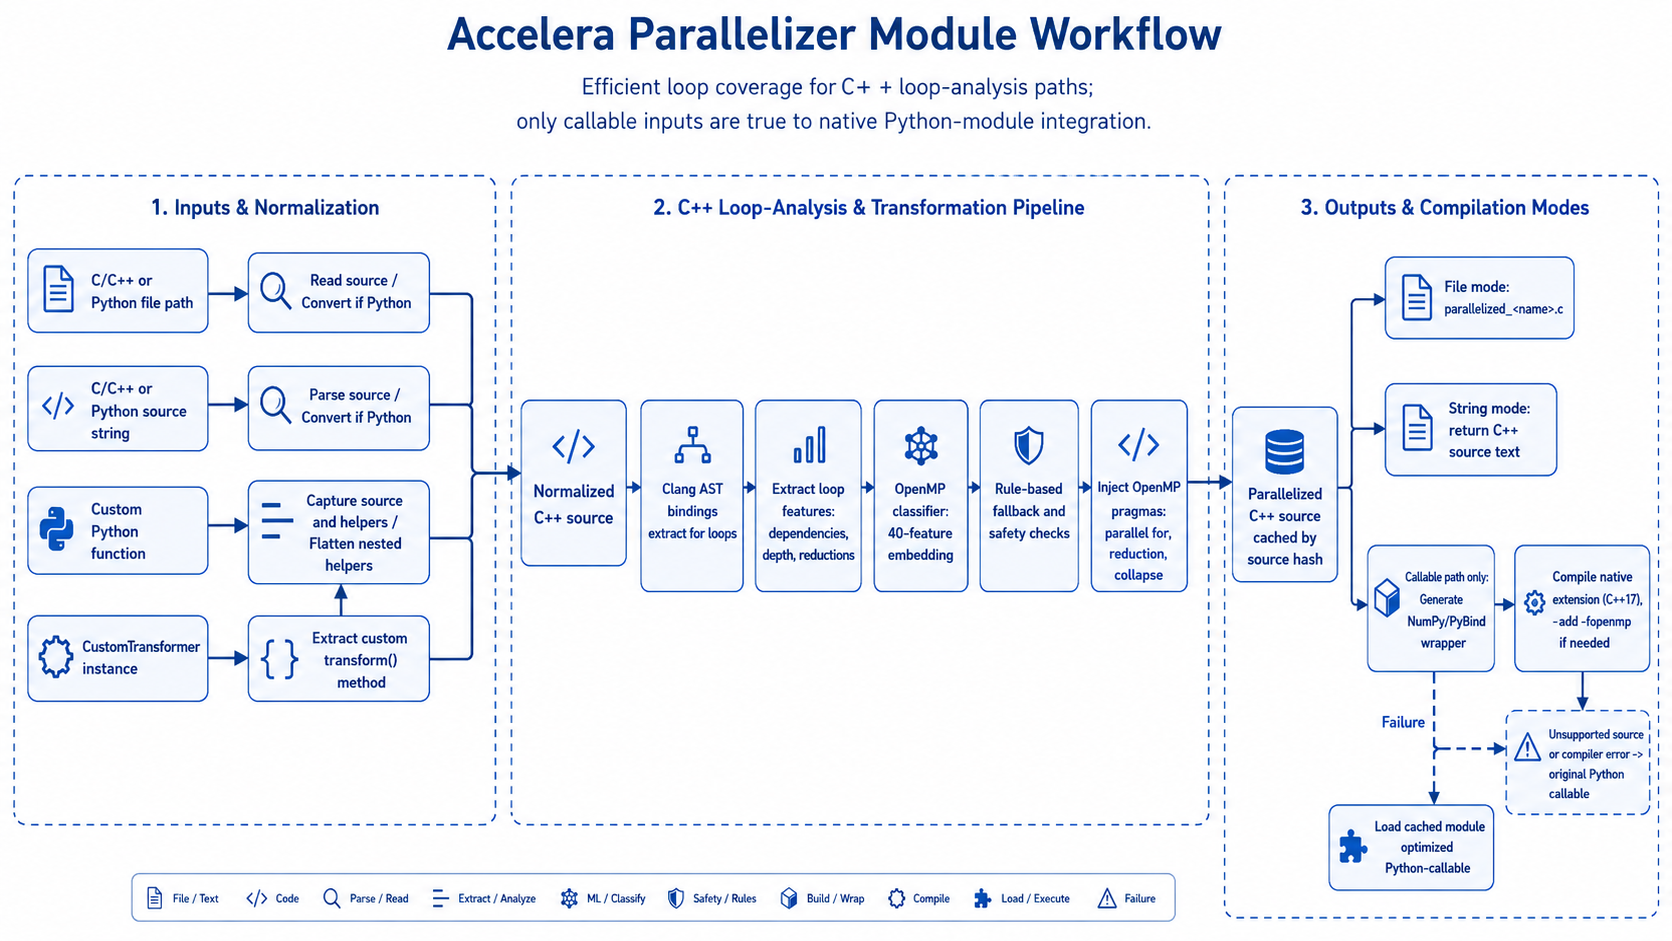
\includegraphics[width=\textwidth,keepaspectratio]{imgs/pp.png}
\caption{Code Parallelizer module workflow}
\label{fig:parallelizer_workflow}
\end{figure}

The feature extraction stage analyzes both code structure and loop behavior, 
including reductions, array accesses, dependencies, indirect memory access, early exits, 
nesting depth, branches, function calls, arithmetic operations, and vectorization potential. 

These indicators are encoded into a 40-dimensional vector for the classifier, 
then refined by deterministic safety rules that can still detect safe cases such as reductions, 
independent array writes, and nested loop patterns.

\begin{lstlisting}[style=algostyle,caption={Loop classification and pragma insertion}]
Input: source program P
Output: source program P' with safe OpenMP pragmas

1:  if P is Python source then
2:      convert the supported Python subset into C++
3:  end if
4:  Extract for-loops using the Clang AST frontend
5:  for each extracted loop L do
6:      compute structural, memory, dependency, and reduction features
7:      send the 40-feature vector to the classifier service
8:      combine the predicted class with rule-based safety checks
9:      if the resolved class is parallel_for then
10:         insert #pragma omp parallel for
11:     else if the resolved class is reduction then
12:         insert #pragma omp parallel for reduction(...)
13:     else
14:         leave the loop unchanged
15:     end if
16: end for
17: Cache and return the transformed source code
\end{lstlisting}

The compilation path is used when the input is a Python callable. The
parallelizer extracts or receives the function source, converts it to C++,
parallelizes the C++ loop body, wraps the result in a PyBind11 module, compiles
it as a shared native extension, loads the extension, and returns the optimized
function. Caching is used at both the transformed-source level and the compiled
method level. The cache key includes the compilation cache version, the function
name, the compiler optimization level, the extension suffix, and the source
code. This prevents recompiling the same function repeatedly.

\subsection{Design Constraints}

The most important design constraint of the Code Parallelizer is correctness.
OpenMP pragmas can improve performance, but an incorrect pragma can produce
wrong numerical results. Therefore, classifier output is not applied blindly.
The module applies additional safety rules to avoid unsafe transformations when
there are loop-carried dependencies, indirect accesses, early exits, side-effect
function calls, or invalid reduction variables. Inner loops are also skipped when
an outer selected loop already covers their range, preventing nested duplicate
pragma insertion.

The second constraint is the restricted Python subset. Full Python semantics are
too dynamic to translate safely into C++ using a lightweight source converter.
The converter therefore rejects unsupported syntax such as decorators, slicing,
chained comparisons, unsupported operators, non-range loop iterators,
multi-target assignment, complex dynamic dispatch, and unsupported expression
forms. This restriction is not a weakness in the design; it is a correctness
boundary. The system optimizes code only when it can produce predictable C++.

The third constraint is compiler and platform compatibility. Native callable
optimization depends on a working C++ compiler, Python include paths, PyBind11
headers, NumPy-compatible array wrapping, and platform-specific shared extension
suffixes. The compiler path uses C++17 and adds \texttt{-fopenmp} only when the
parallelized code actually contains OpenMP pragmas. On non-Windows platforms it
also uses position-independent code flags suitable for shared libraries. If
compilation fails, the original Python callable is returned.

The fourth constraint is input and output compatibility. The current compiled
callable path is oriented toward functions with one named input parameter and
NumPy-like two-dimensional numeric data. The wrapper rewrites array access to
PyBind11 unchecked NumPy access and exposes the compiled function back to
Python. This makes the generated extension useful for numeric preprocessing
loops, but it also means that arbitrary Python functions with complex object
structures are outside the supported optimization target.

The fifth constraint is reproducibility and caching. Because native compilation
can be expensive, the module caches processed C++ code and compiled functions
using source hashes. The cache must include enough information to avoid stale or
incorrect reuse when compiler options, cache version, function name, source code,
or extension suffix changes. This design improves repeated execution time while
keeping cache invalidation explicit.

\subsection{Summary}

The Code Parallelizer is directly integrated with Accelera Pipe. When a
preprocessing node is added, the pipeline calls the parallelizer before storing
the preprocessing object. If the object is a custom Python function, it is wrapped
as a source-backed function whose runtime callable can be replaced by the
compiled implementation. If the object is a custom transformer instance, the
parallelizer attempts to optimize its \texttt{transform} method and attach the
optimized method back to the instance. If the object is a library transformer or
an unsupported callable, it is returned unchanged.

\begin{figure}[H]
\centering
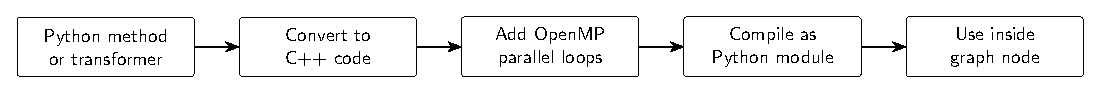
\includegraphics[width=\textwidth]{imgs/parallelizer_accelera_pipe_flow.pdf}
\caption{Integration flow for compiled preprocessing inside Accelera Pipe}
\end{figure}

Scientifically, the final design uses a hybrid approach rather than a purely
generative code model. An earlier generator-based design attempted to emit
parallelized code using a neural sequence model. That approach was rejected
because the dataset size was not sufficient for reliable sequence generation and
because generated synthetic samples risked introducing distribution bias. The
current design is more controlled: the classifier only predicts the type of
parallelization opportunity, while deterministic compiler-like rules decide how
and whether the pragma is inserted. This separation makes the system easier to
inspect, easier to debug, and safer for user code.

Overall, the Code Parallelizer acts as an optimization layer around user-defined
numeric loops. It does not attempt to parallelize all Python programs. Instead,
it targets the subset where static analysis, feature extraction, classifier
prediction, rule validation, and native compilation can cooperate safely. This
fits the broader Accelera design philosophy: keep the Python API simple, but move
performance-sensitive and structurally analyzable work into optimized native
execution when the system can do so without changing program semantics.